\chapter{Lattice gass cellular automata}
The first lattice gass cellular automaton was proposed in 1973 by Hardy, Pomeau and de Pazis \cite{hpp}, and so it is called the HPP model.

Unfortunately, it could not do its job sufficiently well. For the reasons that we will sketch in this chapter, it does not converge to Navier-Stokes equations in macroscopic limit.

\bigskip

In the subsequent chapters we will explore two different approaches how to make functional LGCA. They both build on the idea of this imperfect HPP.

Therefore, we will explain the basic principles of HPP first, and later on, we will upgrade it to FHP, FCHC and our favorite Pair-interaction cellular automaton.

\section{From CA to LGCA}

The lattice of HPP is the simple rectangular 2D grid. At every point of a grid is a node, and this node is composed of 4 cells, see Figure~\ref{rectangular}.

\begin{figure}[htbp]
 \centering
 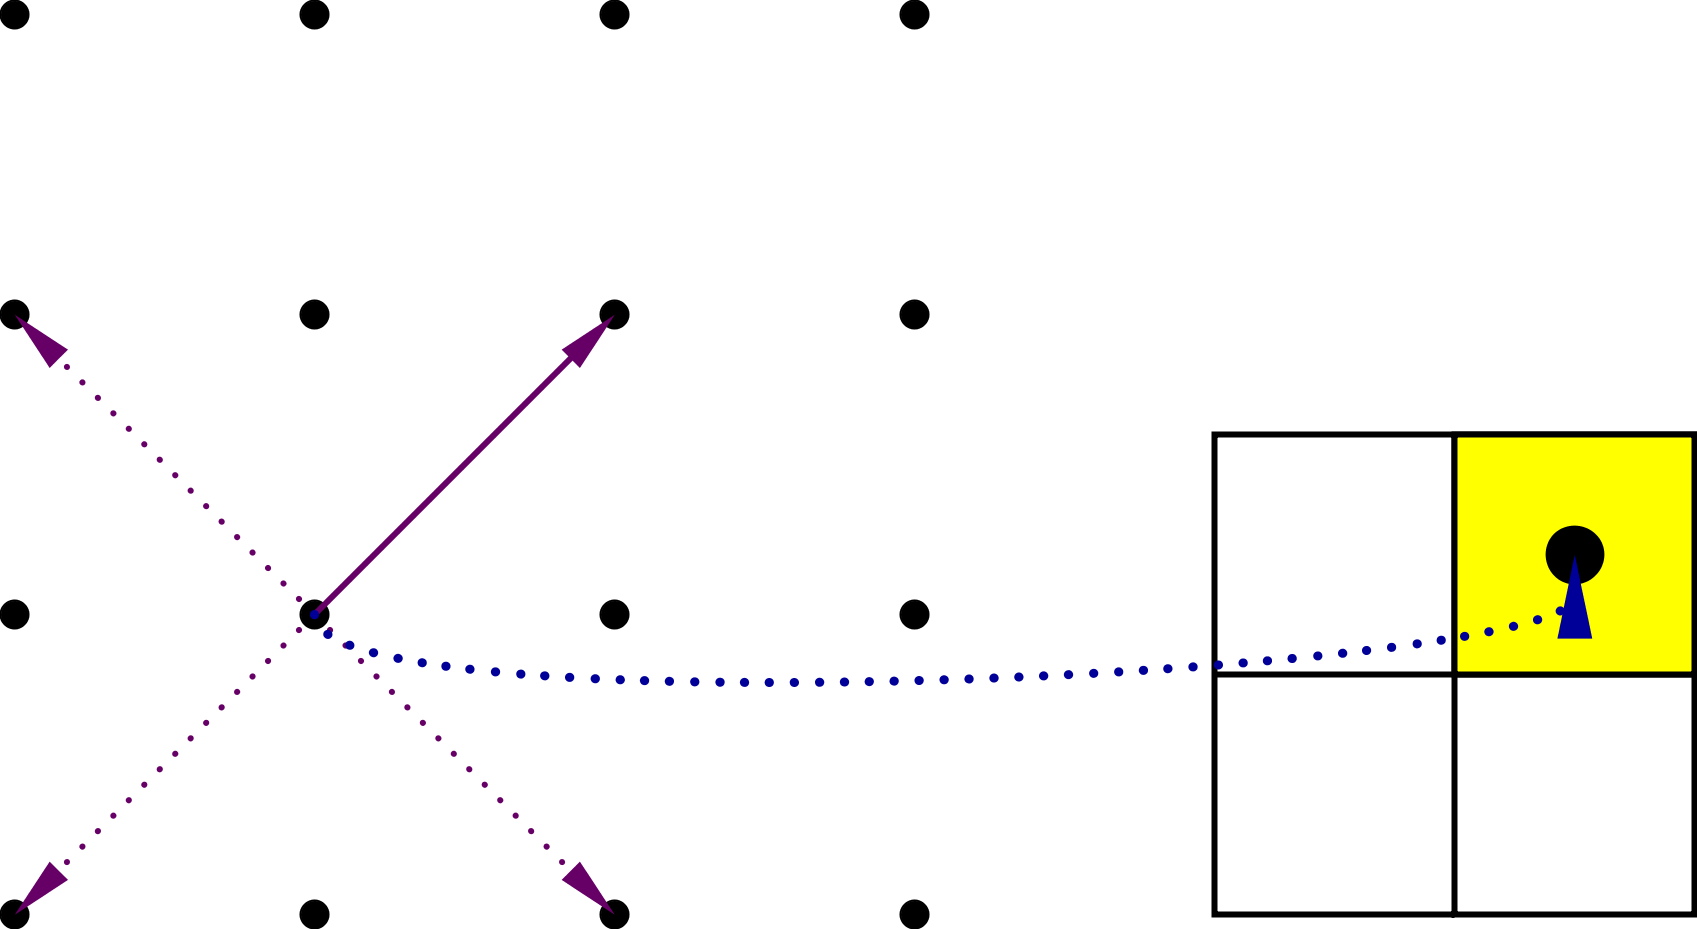
\includegraphics[width=0.6\textwidth]{./img/hppnode}
 \label{rectangular}
 \caption{Rectangular grid}
\end{figure}

Each of these cells can be in two states-- empty (white square) or occupied by the particle (yellow square).
The particle in this cell is heading to the diagonal node along the corresponding lattice vector.

\section{Update rule}
%The update rule should be design in such a manner, that is conserve physically relevant quantities, namely mass and momentum.

At every time-step, the position of the particles is changing in two subsequent steps -- collision and propagation.

During collision, particles are swapped inside the single node, respecting two constraints - number of particle and the total momentum is fixed.

From these constraints follows that there are only two collision configurations for HPP, see Figure~\ref{hpp-colision}.

\begin{figure}[H]
 \centering
 \includegraphics[width=0.7\textwidth]{./img/hpp_col}
 \label{hpp-colision}
 \caption{HPP colisions}
\end{figure}

These configurations are symmetric -- the first one is resolved to the other and vice versa.

%If any other state gets changed, it would break the conservation of momentum and would be physically unrealistic.

\section{Propagation:}

After the collisions are resolved in every node, propagation follows, see Figure \ref{hpp-prop}.
During propagation, particles are streamed along the lattice vectors corresponding to the cells they occupy.
\begin{figure} [H]
 \centering
 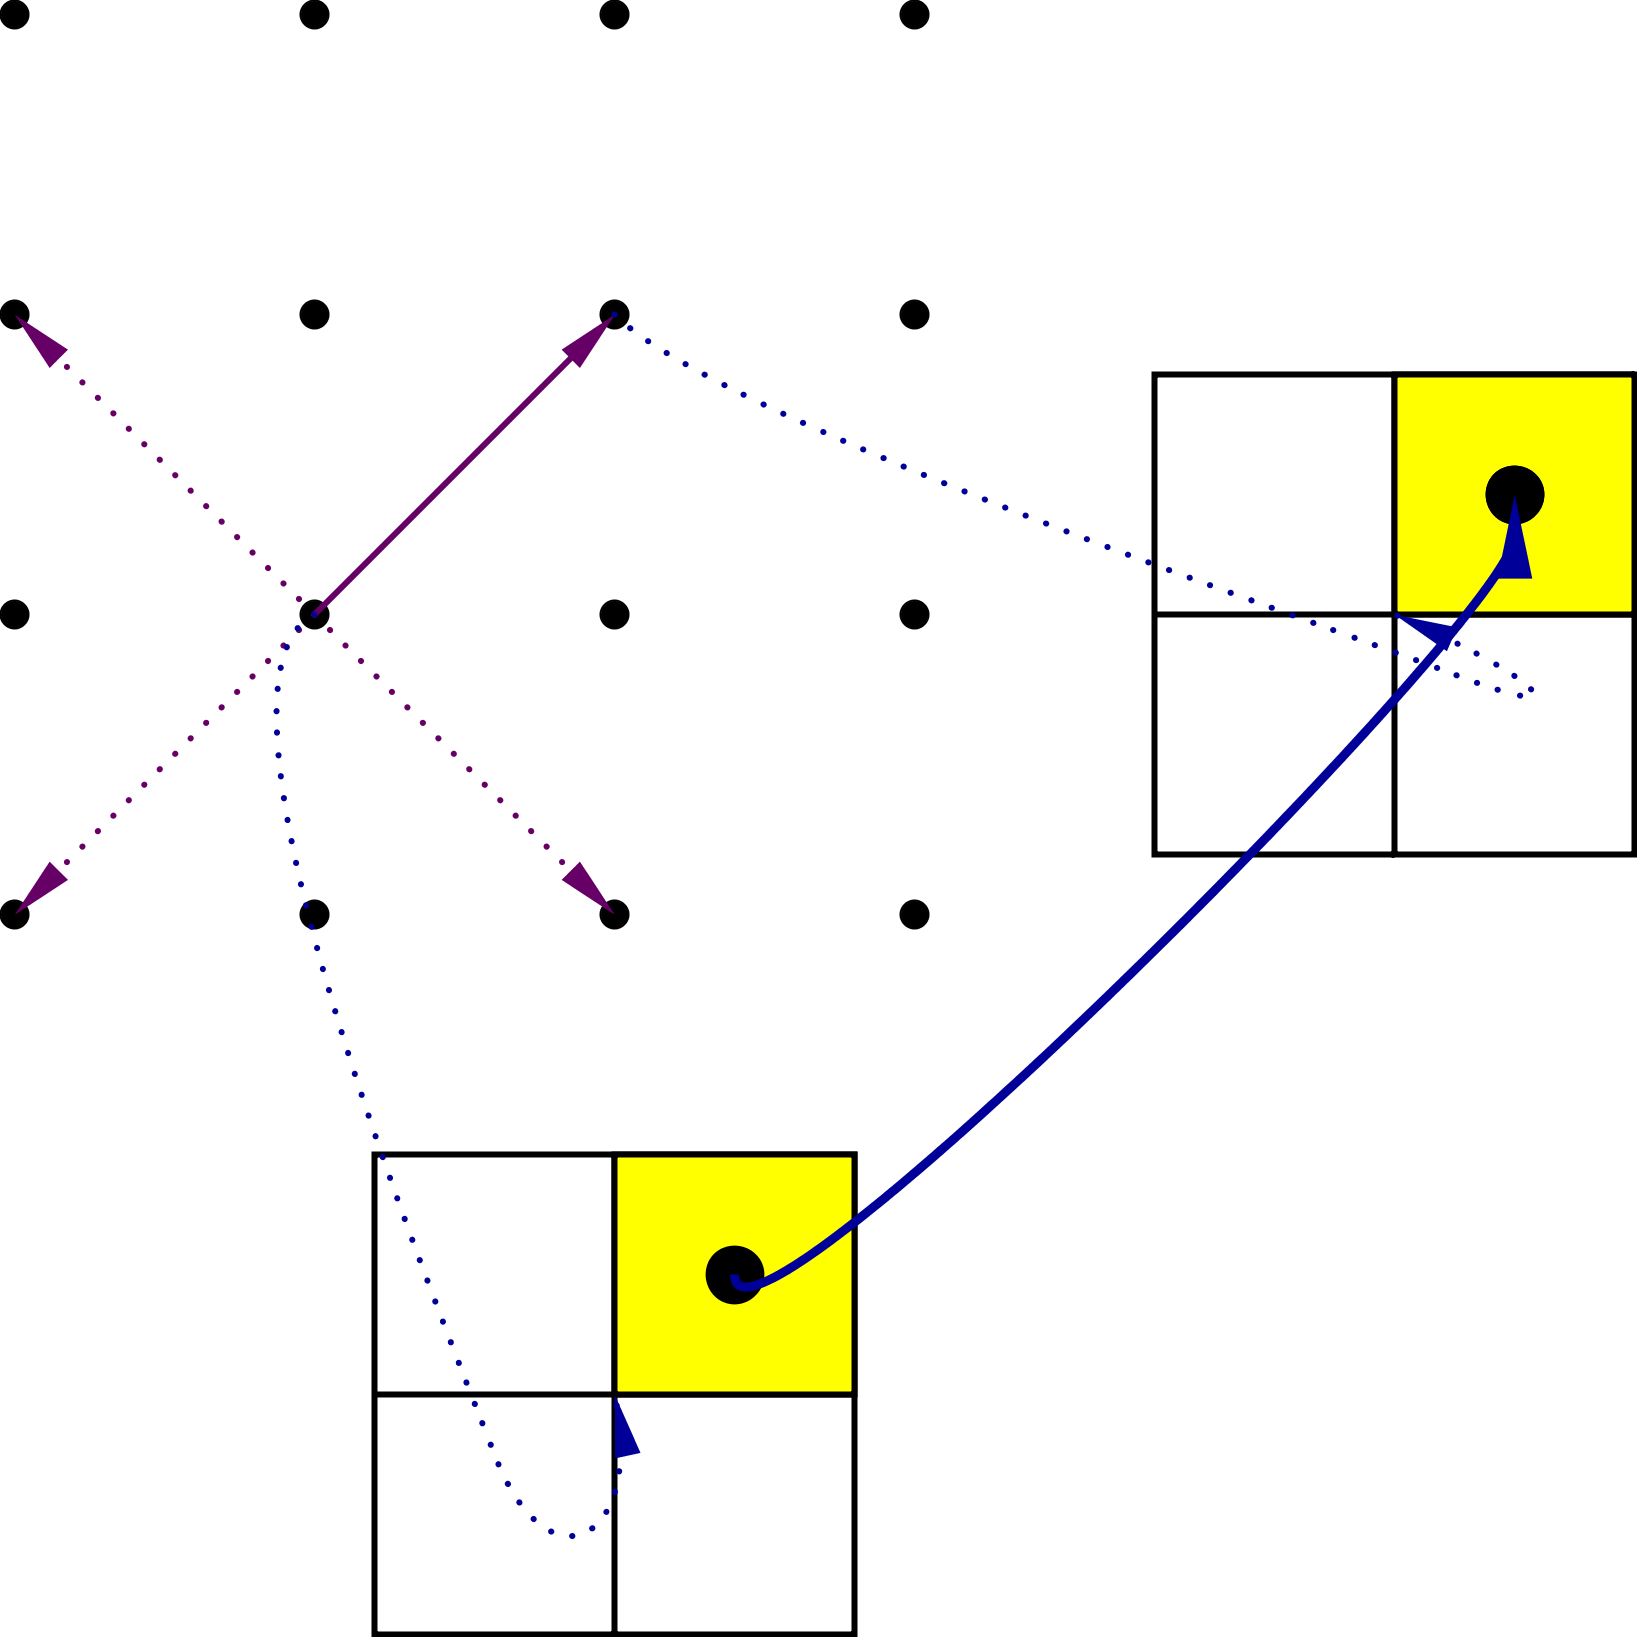
\includegraphics[width=0.6\textwidth]{./img/HPPprop}
 \label{hpp-prop}
 \caption{Propagation of particle from upper-left cell}
\end{figure}

\bigskip

\section{Conservation laws}
 
Let us inspect the mass and momentum conservation of this model in more depth by considering its symmetries.
We assume that lattice is infinite (or finite, but periodic boundary condition are used). Then if we shift the lattice by multiple of lattice vector, we get the same lattice -- the lattice is invariant with respect to translation.
As we know by Norther's theorems, translational symmetry implies conservation of momentum.

Also, the grid possesses a rough rotational symmetry - rotation by the $90\degree$ leads to the same lattice.
However, this rectangular symmetry is not sufficient.
When we will derive the hydrodynamic equations in the following chapter, we may observe that four lattice vectors lead to unrealistic equations, comparing to the models with six and more lattice vectors.

Another problem caused by low rotational symmetry are the non-physical quantities that are conserved nevertheless -- so called spurious invariants \footnote{The improved LGCA also posses the spurious \textit{Zanetti's invariants}, but they are under level of noise, due to higher symmetry and additional collision rules}.

Let us decompose the total momentum of the collision configuration \ref{hpp-colision} into the cardinal directions:
\begin{align} 
P = P_N + P_S + P_E + P_W.
\end{align}
The total momentum $P$ is correctly conserved by the collision, but also quantities
\begin{align} \label{zanet}
P_{spur1} = P_N + P_E - P_S - P_W
\end{align}
and
\begin{align}
P_{spur2} = P_N + P_W - P_S - P_E
\end{align}
are conserved, although these quantities have no physical counterparts.

\section{Conclusion}

To conclude this chapter and finish-off the HPP, it is physically implausible because
\begin{enumerate}
\item angular momentum is not conserved due to insufficient rotational symmetry,
\item other non-physical quantities, so called \textit{spurious invariants} are conserved.
\end{enumerate}

Although it is a flawed model, it sparked interest of the wider community and various successful LGCAs evolved from HPP. In the next chapter, we will introduce the first successful branch of LGCAs -- the FHP model.